% small.tex
\documentclass{beamer}

\newcommand{\RR}{\mathbb{R}}
\newcommand{\ra}{\rightarrow}
\newcommand{\Wo}{W^{(1)}}
\newcommand{\Wt}{W^{(2)}}
\newcommand{\bo}{b^{(1)}}
\newcommand{\bt}{b^{(2)}}
\newcommand{\zr}{z^{(3)}}
\newcommand{\zt}{z^{(2)}}
\newcommand{\ar}{a^{(3)}}
\newcommand{\at}{a^{(2)}}
\newcommand{\ao}{a^{(1)}}
\newcommand{\dr}{\delta^{(3)}}
\newcommand{\dt}{\delta^{(2)}}
\newcommand{\xii}{x^{(i)}}
\newcommand{\pd}[2]{\ensuremath{\cfrac{\partial #1}{\partial #2}}}

\usetheme{default}
\begin{document}

\begin{frame}{Sparse Autoencoders}

Autoencoders are neural networks that try to learn the identity function.
Sparsity constraints force the learned representation to be nontrivial.

\begin{figure}[htb]
\begin{center}
\label{proc_sched}
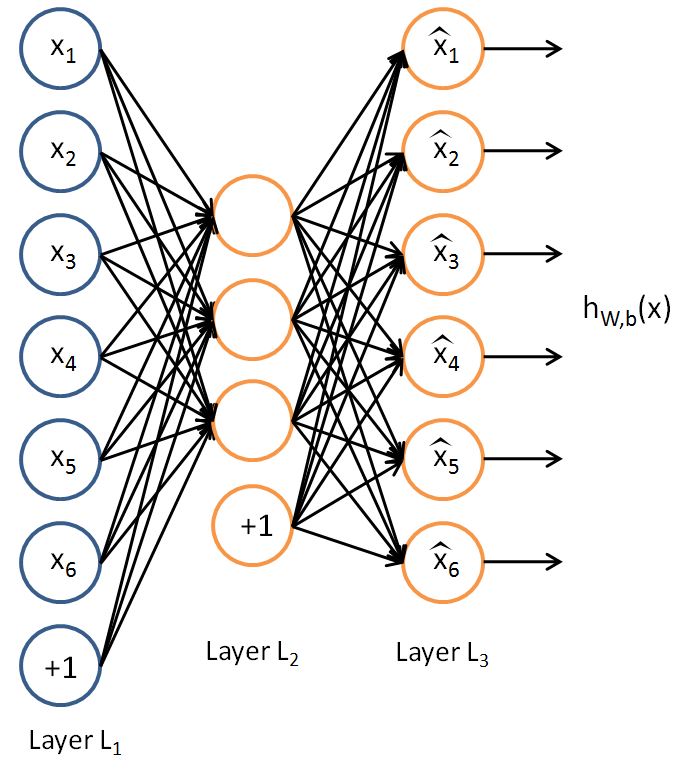
\includegraphics[width=0.5\textwidth]{Autoencoder636.png}
\caption{Autoencoder}
\end{center}
\end{figure}

\end{frame}
\begin{frame}{Cost Function}
\small
Let the hidden layer have $p$ units, and let $f:\RR\ra\RR$ be a differentiable
activation function. The neural network is parameterized by terms weights
$\Wo\in\RR^{p\times n}$ and $\Wt\in\RR^{n\times p}$ and bias terms $\bo\in\RR^p$
and $\bt\in\RR^n$. The prediction on an input
$x\in\RR^n$ is
\[h_{W,b}=f(\Wt f(\Wo x+\bo)+\bt)\]
Given training examples $x^{(1)},\ldots,x^{(m)}\in\RR^n$ the objective function is
\[J(W,b)=\frac1m\sum_{i=1}^m\ell(h_{W,b}(\xii),\xii)+\lambda\psi(W,b)+\beta\sum_{j=1}^p\phi(\hat\rho_j)\]
where 
\[\hat\rho_j=\frac1m\sum_{j=1}^mf\left((\Wo_j)^T\xii+\bo_j\right)\] is 
the average activation of the $j$th hidden unit over the training set and $\ell:\RR^n\times\RR^n\ra\RR$ is a loss function. The function
$\psi$ is a regularizer.
\normalsize
\end{frame}
\begin{frame}{A sample slide}

A displayed formula:

\[
  \int_{-\infty}^\infty e^{-x^2} \, dx = \sqrt{\pi}
  \]

An itemized list:

\begin{itemize}
\item itemized item 1
\item itemized item 2
\item itemized item 3
\end{itemize}

\begin{theorem}
In a right triangle, the square of hypotenuse equals
the sum of squares of two other sides.
\end{theorem}
\end{frame}

\end{document}
